\subsection{ChatterBot MathBot (do Discord)}\label{subsec:bot3} 

Esse MathBot (possui o mesmo nome que o bot anterior) é outro sistema implementado na linguagem Python e desenvolvido para o aplicativo Discord\footnote{Discord é um aplicativo de voz sobre IP proprietário e gratuito, projetado para comunidades de jogos~\cite{wiki_discord}. Está disponível no site \url{www.discordapp.com}} com o bordão ``Mathematics For Discord''.
Em seu site (\url{www.dxsmiley.github.io}) possui instruções para uso e documenta suas funcionalidades, que são:
executar \emph{querys} do Wolfram\textbar Alpha\footnote{Wolfram\textbar Alpha é um mecanismo de conhecimento computacional. É um serviço on-line que responde às perguntas diretamente, mediante o processamento da resposta extraída de base de dados estruturados, em lugar de proporcionar uma lista dos documentos ou páginas web que poderiam conter a resposta, tal como faziam os mecanismos de busca~\cite{wiki_wolfram}.},
renderizar textos em \LaTeX{}, realizar operações lógicas e aritméticas (além de cálculos mais complexos), entre outras.

Para testá-lo e analisá-lo, me concentrei nas funções de calculadora que ele propõe. 
O bot possui uma postura unidirecional, assim, para iniciar a conversa, basta enviar a informação que você deseja seguindo os padrões documentados.
O texto e a imagem a seguir mostram a interação inicial com o bot:
\begin{description}
    \item \eu{=calc sin(pi / 2)}
    \item \chatbot{1}
    \item \eu{=wolf plot cosh\textasciicircum2(x)}
\end{description}
\begin{figure}[h!tbp]
    \centering
    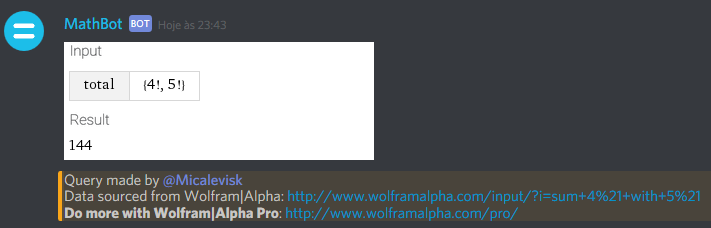
\includegraphics[width=1\linewidth]{img/bot3_1.png}
    % \caption{Screenshot da resposta do MathBot (do Discord).}
    \label{fig:bot3_1}
\end{figure}

Quando a mensagem do usuário se inicia com o texto ``=wolf'', o bot entende que deve utilizar a API do sistema Wolfram Alpha para executar a \emph{query} do usuário (que vem a seguir). A mensagem de resposta é uma (ou mais) imagem, seguida dos links de origem da imagem. Além disso, com o uso desse sistema, é possível enviar mensagens como ``sum 1 with 1'' que serão compreendidas.